% This file was created with tikzplotlib v0.10.1.
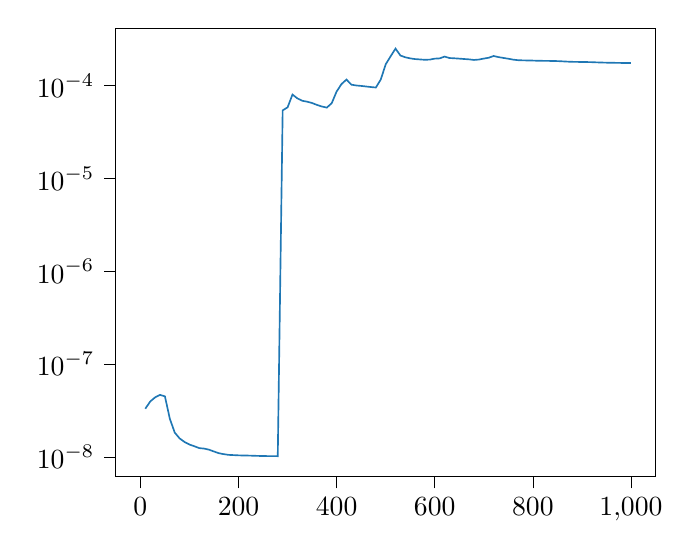
\begin{tikzpicture}

\definecolor{darkgray176}{RGB}{176,176,176}
\definecolor{steelblue31119180}{RGB}{31,119,180}

\begin{axis}[
log basis y={10},
tick align=outside,
tick pos=left,
x grid style={darkgray176},
xmin=-50, xmax=1050,
xtick style={color=black},
y grid style={darkgray176},
ymin=6.12177401299148e-09, ymax=0.000417036434333516,
ymode=log,
ytick style={color=black},
ytick={1e-10,1e-09,1e-08,1e-07,1e-06,1e-05,0.0001,0.001,0.01},
yticklabels={
  \(\displaystyle {10^{-10}}\),
  \(\displaystyle {10^{-9}}\),
  \(\displaystyle {10^{-8}}\),
  \(\displaystyle {10^{-7}}\),
  \(\displaystyle {10^{-6}}\),
  \(\displaystyle {10^{-5}}\),
  \(\displaystyle {10^{-4}}\),
  \(\displaystyle {10^{-3}}\),
  \(\displaystyle {10^{-2}}\)
}
]
\addplot [semithick, steelblue31119180]
table {%
10 3.29570816374376e-08
20 3.94528057808657e-08
30 4.37160664750453e-08
40 4.64847742939375e-08
50 4.4805614268671e-08
60 2.56793092271618e-08
70 1.82290994250967e-08
80 1.57719376960663e-08
90 1.44379659116728e-08
100 1.35562135200414e-08
110 1.2988295745061e-08
120 1.23998964962538e-08
130 1.22517631931338e-08
140 1.19192784763798e-08
150 1.13949870525143e-08
160 1.09222598246694e-08
170 1.06719262701527e-08
180 1.04851520885914e-08
190 1.04203167194874e-08
200 1.0360297749445e-08
210 1.03219694642325e-08
220 1.0302645793246e-08
230 1.02653299665269e-08
240 1.02212585250318e-08
250 1.01905315979051e-08
260 1.01693157067369e-08
270 1.01563203497066e-08
280 1.01524906509993e-08
290 5.42686962498327e-05
300 5.8518984322748e-05
310 8.03588664150051e-05
320 7.30752460901305e-05
330 6.88722287387102e-05
340 6.72988082772348e-05
350 6.51634901148979e-05
360 6.2098144321965e-05
370 5.97352365927694e-05
380 5.81243403663653e-05
390 6.48833938664201e-05
400 8.67858560531903e-05
410 0.00010438064631096
420 0.000116628392728912
430 0.000102713537931062
440 0.000100680417153614
450 9.95967240439967e-05
460 9.82037216895446e-05
470 9.68366513171482e-05
480 9.57143171726728e-05
490 0.000116830510161037
500 0.000170302639285684
510 0.000207536758068608
520 0.000251465664331566
530 0.000211914684729464
540 0.000202730334759811
550 0.000197380313134692
560 0.000193903789625457
570 0.000192166235454706
580 0.000190542191182592
590 0.000191540573783065
600 0.000196027377812374
610 0.000197245675473921
620 0.000206405137331648
630 0.00019901554612504
640 0.000197776940739523
650 0.000196095335055934
660 0.000194234164710475
670 0.000192552234475035
680 0.000189761480791291
690 0.000191679382479177
700 0.000196393780594774
710 0.000200463368116177
720 0.000209332076116129
730 0.000203614233271165
740 0.000199485202854981
750 0.000195605126446786
760 0.000191197660764221
770 0.000188682780714902
780 0.000187793784687984
790 0.000187371472930892
800 0.000186818425204526
810 0.000186046516147132
820 0.000185674215279702
830 0.000185419334303972
840 0.000185054986352275
850 0.000184428613705405
860 0.000183331455730868
870 0.000182065044658081
880 0.00018117719192377
890 0.000180807186123732
900 0.000180480614750017
910 0.000180115302687573
920 0.00017957976344544
930 0.000178729404619659
940 0.000177982800233641
950 0.000177376920490995
960 0.000176937103969059
970 0.000176591711576117
980 0.000176265831581719
990 0.000176042482816276
1000 0.000175911019008011
};
\path [draw=black, semithick, dash pattern=on 5.55pt off 2.4pt]
(axis cs:0,0)
--(axis cs:1000,0);

\end{axis}

\end{tikzpicture}
